\documentclass[conference]{IEEEtran}
\IEEEoverridecommandlockouts
% The preceding line is only needed to identify funding in the first footnote. If that is unneeded, please comment it out.
\usepackage{cite}
\usepackage[utf8]{inputenc}
\usepackage[english]{babel}
\usepackage{amsmath,amssymb,amsfonts}
\usepackage{algorithmic}
\usepackage{graphicx}
\usepackage{textcomp}
\usepackage{listings}
\usepackage{xcolor}
\usepackage{tabularx}
\usepackage{hyperref}

% import packages: "caption" "subfig" - according to "A. Figures 1)"

\ifCLASSOPTIONcompsoc
\usepackage[caption=false,font=normalsize,labelfont=sf,textfont=sf]{subfig}
\else
\usepackage[caption=false,font=footnotesize]{subfig}
\fi

\usepackage{ dsfont }
\definecolor{gray}{gray}{0.9}
\def\BibTeX{{\rm B\kern-.05em{\sc i\kern-.025em b}\kern-.08em
    T\kern-.1667em\lower.7ex\hbox{E}\kern-.125emX}}

\pagenumbering{arabic}
\usepackage{fancyhdr}
\usepackage{lastpage}
\pagestyle{fancy}
\fancyhf{}

\begin{document}

% title with \title and maketitle according to section "A. Paper Title"

\title{Learning to play RoboSkate with reinforcement learning}

% authors according to section "B. Author Names"

\author{
\IEEEauthorblockN{Finn Süberkrüb, Gintautas Palinauskas, Meric Sakarya, Michelle Bettendorf, Batuhan Yumurtaci\\\\}

\IEEEauthorblockA{Chair of Robotics, Artificial Intelligence and Real-time Systems\\
TUM Department of Informatics\\
Technical University of Munich\\\\
finn.sueberkrueb@tum.de, gintautas.palinauskas@tum.de, meric.sakarya@tum.de, michelle.bettendorf@tum.de,\\ batuhan.yumurtaci@tum.de}}

\maketitle

% for page numberring https://newbedev.com/forcing-page-numbers-with-ieeetran
\thispagestyle{plain}
\pagestyle{plain}

% abstract and keywords according to "V. A BSTRACT AND INDEX TERMS"

\begin{abstract}
An OpenAI Gym Environment was designed to train a reinforcement learning agent on the Unity game RoboSkate using a custom policy that on different levels combines camera data with numerical observations and uses a soft actor critic for learning.\\
\end{abstract}

\begin{IEEEkeywords}
RoboSkate, Unity, Reinforcement Learning, Imitation Learning, SAC, PPO, A2C, VAE, AI, SB3
\end{IEEEkeywords}

\tableofcontents

% ========= Whole text info  =========
% "figure" replaced with \figurename according to section "A. Figures"
% citations with \cite according to section "VII. CITATIONS"
% start of section with \section , \subsection , \subsubsection according to section "VI. SECTIONS"
% Figures according to "A. Figures"


% Changed first word style according to section "A. Initial Drop Cap Letter"

\section{Introduction}
\IEEEPARstart{R}{oboSkate} is a game where a 3R manipulator is centrally mounted on a skateboard \cite{RoboSkate} and controlled by a player it must navigate through a parkour track and reach the finish line. Because of it's unintuitive control it has a steep learning curve for beginners. That's why it is interesting to apply AI to the game. In the following technical report several approaches are described that led to a successfully trained RoboSkate agent that can keep up with the most experienced human players.


\section{Unity as OpenAI Gym environment}
Unity games offer interesting possibilities like realistic environments, physics simulations as an environment for reinforcement learning. At the same time, it raises some difficulties when executing on servers, because Unity is designed to run on a graphical desktop.

\subsection{Unity "headless" mode}
There is an option to build and run Unity games in "headless" mode \cite{unityHeadless}, which allows to run them without graphical output and use the physics engine to its full extent. But as a consequence it is not allowed
to render. Therefore, it is only suitable for problems without image data. 

\subsection{Unity WebGL}
It is also possible to build Unity games using WebGL. These can be easily launched from a server and run in the browser. However, this solution does not support gRPC communication, which is the middleware used in our case.

\subsection{Unity machine learning agents}
This tool allows training agents directly inside Unity. Parallel training is realized by several games in the same Unity scene \cite{unityRL}.

\subsection{Unity game without monitor}
The most interesting variant, however, is when running unity games directly on the system \cite{unitywithoutMonitor}. To run Unity games in Docker containers, three components are required:

% list according to "A. Itemize"

\begin{itemize}
    \item NVIDIA container runtime \cite{nvidiagpucontainersruntime}
    \item Dummy XServer \cite{ServerGUI}
    \item Vulkan engine \cite{nvidiavulkan}
\end{itemize}
To get started, XServer must be configured after the installation and started together with the RoboSkate game on the appropriate dummy monitor.

\section{RoboSkate Agent}  \label{RoboSkate_Agent}
The RoboSkate agent consists of a skateboard with a 3R robotic arm. It is viewed from a third person's perspective (\figurename  \ref{fig:RoboSkate_agent}).

\subsection{Action space}
The action space consists of three parameters, each controlling the forces applied to the individual joints. There is no predefined limit for them. If a sufficiently large force is applied to joint 1 for a long time, it accelerates until the graphical representation of Unity has problems with the calculation.

Joint force values in the range [-40; 40] are well suited for permanent application, higher values were observed to be unstable in there numerical representation. Since the arm is simulated with a physical mass, a higher force can be used for a short time, since the inertia limits the acceleration at that moment.

\begin{figure}[!t]
  \centering
  \includegraphics[width=.9\linewidth]{images/RoboSkateBord.png}
  \caption{RoboSkate agent with fixed camera position.}
  \label{fig:RoboSkate_agent}
\end{figure}

\subsection{Observation space}
All observations that are accessible from the Unity RoboSkate game are listed in table \ref{tab:all_observation}. For example, two vectors are given for the board rotation relative to the world coordinate system. The first vector describes the "forward" direction of the robot in world coordinates. The second vector - the "upward" direction. See the examples in table \ref{tab:all_observation} for more detail.


\section{Reinforcement learning architecture}
\figurename  \ref{fig:RL_agent} shows the structure of the used RL agent. The used observations fulfill the Markov property to a sufficient degree. Acceleration values were not used because their numerical representations were unstable. The position of the robot was also not used to avoid the agent from learning the route by heart. Same is true for the orientation along the vertical axis (yaw).
Furthermore, the observation space was reduced for faster training. Only one forward velocity vector was used as well as the two Euler angles roll and pitch.

In the following $F_x$ denotes the $x$ component of the vector which points from the board to the front (In table \ref{tab:all_observation} boardRotation[7]). $\vec{U}$ is the vector which points upwards and $ \vec{L} = \vec{F} \times \vec{U} $ is the cross product which results in the orthogonal third vector to span $\mathds{R}^3$. $P$ denotes the position vector of the robot relative to the world coordinate system in $x, y, z $ coordinates. %\underline{\#Gin: Why board velocity is not div of P ? Importent!\#}

% equations according to the rules section "VIII. EQUATIONS"

\begin{equation}
\text{board yaw} = \tan ^{-1} \frac{F_y}{F_x}
\end{equation}

\begin{equation}
\text{board pitch} = \tan ^{-1} \frac{\lVert [F_x , F_y]^T \rVert}{F_z}
\end{equation}

\begin{equation}
\text{board roll} = \tan ^{-1} \frac{\lVert [L_x , L_y]^T \rVert}{L_z}
\end{equation}

\begin{equation}
\text{board velocity} = [\dot{P}_x , \dot{P}_y]^T
\end{equation}

\begin{figure}[ht]
  \centering
  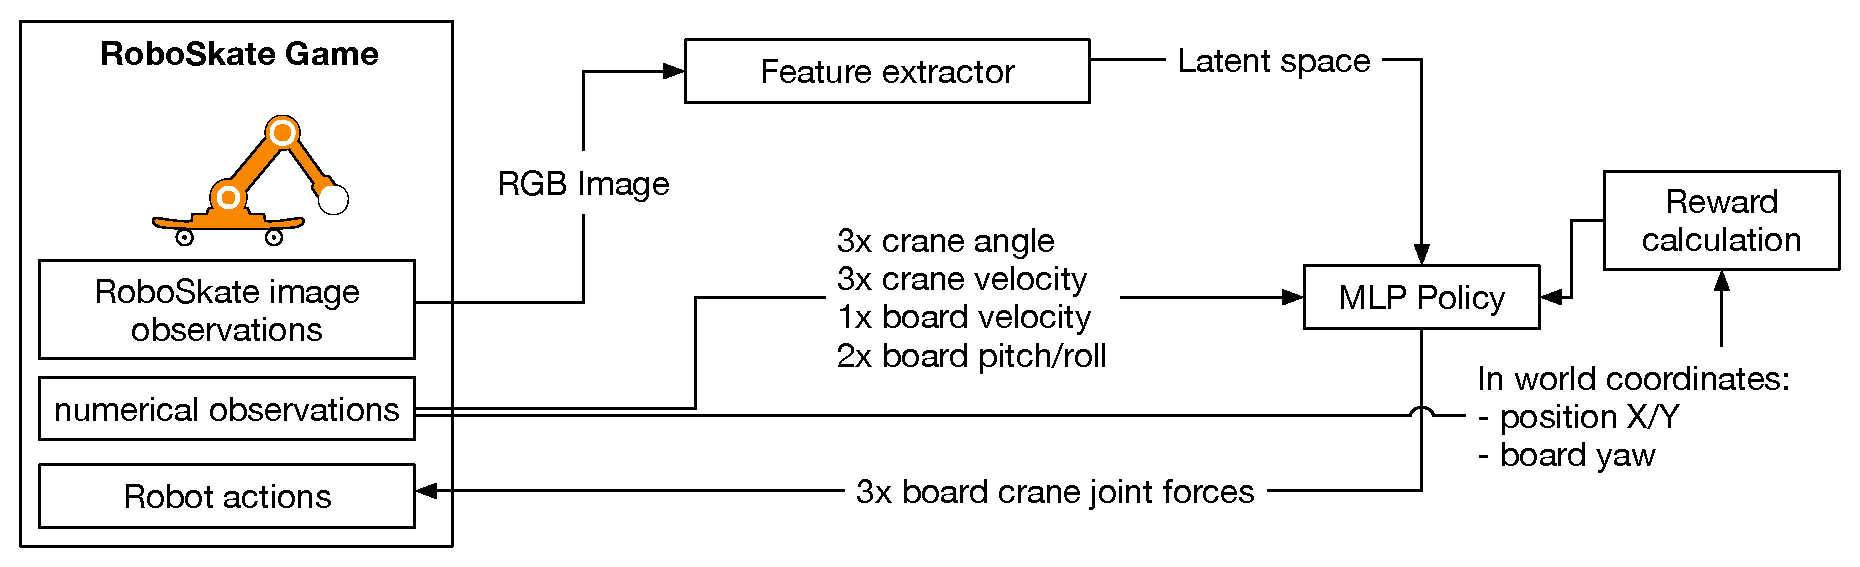
\includegraphics[width=1.0\linewidth]{images/RL_agent.eps}
  \caption{Used reinforcement learning agent.}
\label{fig:RL_agent}
\end{figure}

To combine image data with numerical data, several feature extractors have been developed which are described below. The image features were then stacked with the numerical observations and provided to the policy. In the first case where the image features have been replaced by a single steering angle, the policy is shown in \figurename  \ref{fig:MLP_Policy}. The same policy is also used when the latent space of the feature extractor is larger. The only adjustment is the size of the input layer.


\begin{figure}[!t]
  \centering
  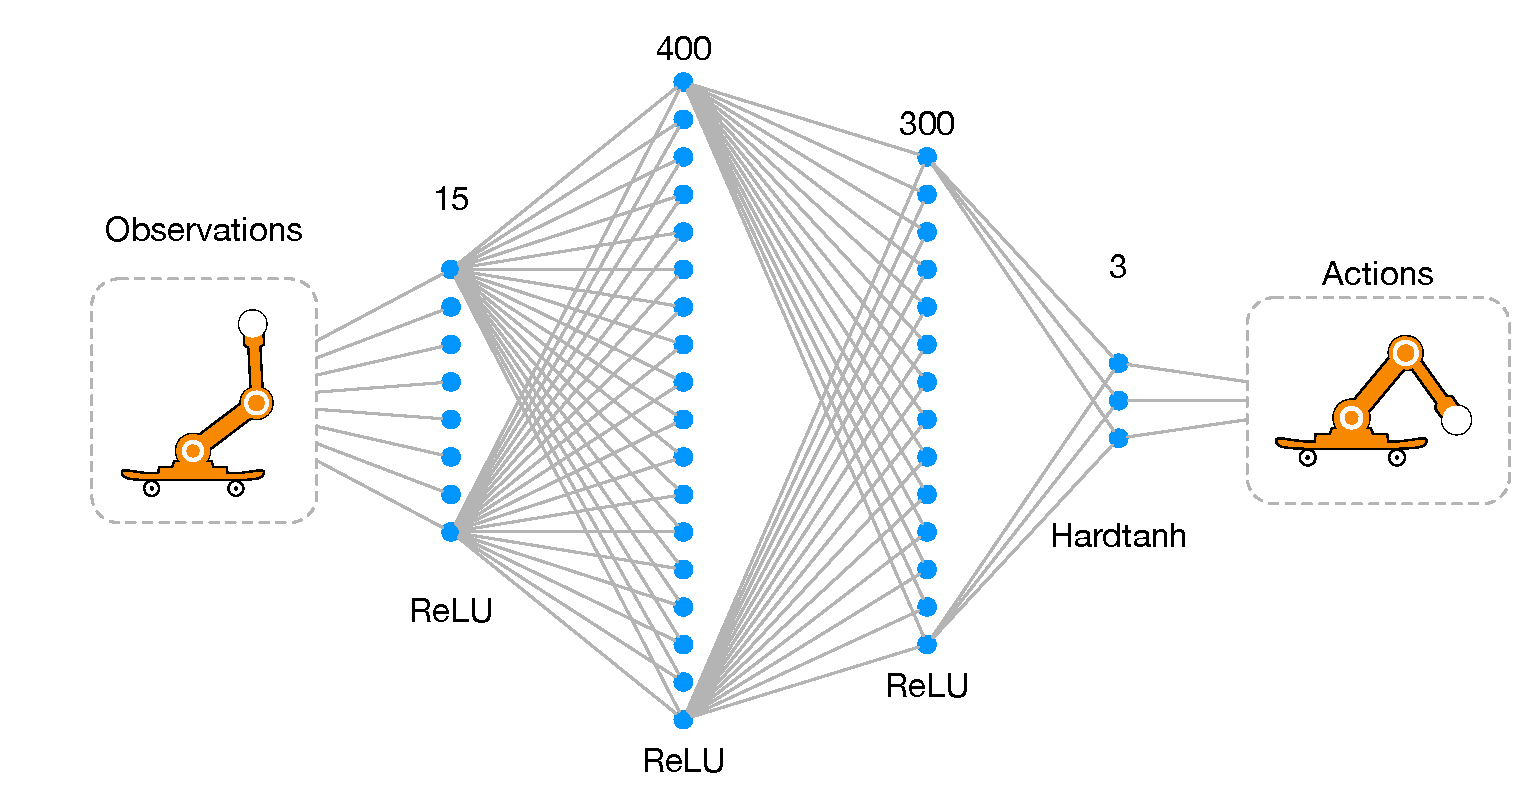
\includegraphics[width=1.0\linewidth]{images/SAC_MLP_Policy.eps}
  \caption{Policy for learning from numerical Data and optimal steering angle.}
\label{fig:MLP_Policy}
\end{figure}



\subsection{Reward function}
The reward function is based on a list of checkpoints (\figurename  \ref{fig:Checkpoint_map}). Depending on the start level, a corresponding checkpoint is loaded. As soon as the agent has reached the certain radius of the checkpoint, the next point is set as the target.
For each step a reward proportional to the distance $x$ and the angle $\alpha$ is assigned (\figurename  \ref{fig:Reward_keep_line}). The distance $x$ is the distance covered during the step in the direction of the next checkpoint. The angle $\alpha$ (in degrees) indicates how the orientation was improved towards the checkpoint. Both values are negative when moving/rotating in the wrong direction.

% equations according to the rules section "VIII. EQUATIONS"

\begin{equation}
\text{reward} = 5x + 1\alpha
\end{equation}

Another part that initially played an important role in the reward function was the negative distance of the end effector to the ground (\figurename  \ref{fig:Reward_low_ball}). This helped guiding the search in the right direction and accelerated the learning process in the beginning. It turned out that a modified initialization of the robot, where the arm starts directly with ground contact, also accelerates the learning and at the same time does not constrain the later actions e.g. for steering. In the game, the robot is usually initialized with the arm pointing straight upwards. This initialization can be used again after training to create equal starting conditions for comparisons between humans and agents.


\begin{figure}[!t]
  \centering
  \includegraphics[width=1\linewidth]{images/RoboSkate_Map.eps}
  \caption{Checkpoints with acceptance radius.}
\label{fig:Checkpoint_map}
\end{figure}


\begin{figure}[!t]
  \centering
  \includegraphics[width=1\linewidth]{images/checkpoint_reward.eps}
  \caption{Reward for traveled distance $x$ and corrected orientation $\alpha$ to the next checkpoint.}
\label{fig:Reward_keep_line}
\end{figure}


\begin{figure}[!t]
  \centering
  \includegraphics[width=0.8\linewidth]{images/Reward_low_ball.jpg}
  \caption{Reward for low arm / different starting position.}
\label{fig:Reward_low_ball}
\end{figure}

\subsection{Termination conditions} \label{Termination_conditions}
In addition to the reward function, there are further termination conditions that can end an episode:

% list according to "B. Enumerate"

\begin{enumerate}[\IEEEsetlabelwidth{5}]
    \item Dropping from the platform
    \item Skateboard falling over
    \item Consistently too high action values on joint 1 
    \item Reaching maximum number of steps
    \item Reaching the last checkpoint
\end{enumerate}
 They would result in an extra reward or punishment. Note the third point is required to avoid simulation glitches.

\subsection{Environment with steering angle}   \label{Environment_steering_angle}
There are two processes that need to be learned: path planning from images and locomotion from given directions. In order to decouple the learning, in the first step the agent is provided with the optimal steering angle at the current robot position and rotation. The deviation from the optimal trajectory, defined by checkpoints, is then calculated and an angle is returned. This information will later be replaced by the image data. Because the environment provides the angle, an agent without image information can be trained in the first step, which simplifies the problem significantly and also reduces the requirements on the computing machine (no GPU needed).

\subsection{SAC}
The first successful training experiment without image data was performed with the SAC \cite{haarnoja2018soft} implementation of Stable Baselines-3 \cite{SB3}. All training parameters are shown in Table \ref{table:SACparams}.

% tables according to "C. Tables"

\begin{table}[!t]
\renewcommand{\arraystretch}{1.3}
\caption{Parameters for SAC training}
\label{table:SACparams}
\centering
\begin{tabularx}{0.45\textwidth} { 
  | >{\raggedright\arraybackslash}X 
  >{\raggedleft\arraybackslash}X |}
 \hline
 Parameter & Value\\
 \hline
 number of timesteps & 0.75M\\
 learning rate & 0.00073\\
 buffer size & 300000\\
 batch size & 256\\
 discount factor & 0.98\\
 Actor network structure & FC 256 - FC 256 - FC (Out)\\
 Critic network structure & FC 256 - FC 256 - FC 1\\
 Activation functions & ReLU\\
 optimizer & Adam (lr = 0.00073)\\
 RoboSkate Level & 1\\
 \hline
\end{tabularx}
\medskip
\end{table}

The agent generalizes very well, so that e.g. level 3 can be solved, when trained on level 2. Level 1 has the difficulty of a slope and a step, since such conditions do not occur in the other levels, an agent trained on level 2 can usually not solve level 1 so well.

In the learning curve for Level 2, \figurename  \ref{fig:SAC01learningcurv}, it can be seen how the agent first learns to finish the level and then improves its movements so that it solves the level in almost half the time it took at the beginning. 400k training steps took 8 hours in the used setting.

A video of the fully trained agent can be found here: https://youtu.be/fPrDSwJhh1M.

% Subfigures according to "A. Figures 1)"

\begin{figure}[!t]
\centering
\subfloat[mean reward.]{\includegraphics[width=0.2\textwidth]{images/Level_1-3_ep_rew_mean.eps}}
\hfil
\subfloat[mean episode length.]{\includegraphics[width=0.2\textwidth]{images/Level_1-3_ep_len_mean.eps}}
\caption{SAC training curves numerical agent.}
\label{fig:SAC01learningcurv}
\end{figure}


\subsection{PPO and A2C}
The PPO \cite{schulman2017proximal} and A2C \cite{mnih2016asynchronous} algorithms from Stable Baselines-3 were also explored. However, since the RoboSkate game is very resource intensive the number of parallel running game instances is very limited. Therefore the number of parallel environments used in on-policy algorithms could not keep up with the replay buffer of the SAC implementation (\figurename  \ref{fig:PPO_and_A2C}).
%In the case of numerical observations, two servers could be combined in order to train up to 20 environments simultaneously \underline{\#Gin: Guess it depends on the servers?\#}.
In our case only one server was equipped with GPUs and these were needed for the RoboSkate game to train with image data, therefore A2C and PPO were excluded from further attempts.

\begin{figure}[!t]
  \centering
  \includegraphics[width=0.8\linewidth]{images/Trainings_algorithm_comparison.eps}
  \caption{Training comparison between different algorithms for numerical observations. Reward cannot be compared with other trainings because of different weightings.}
\label{fig:PPO_and_A2C}
\end{figure}


\section{Imitation Learning}
\subsection{Hardcoded agent} \label{Hardcoded_agent}
To make imitation learning possible, expert data is required that was generated by a hardcoded agent. Since the agent is very difficult to control for an inexperienced player, a control was implemented which generates an arm movement from steering instructions. The controller has a fully-automatic mode in which it follows waypoints and a semi-automatic mode in which the direction is given by a user.

\begin{figure}[!t]
  \centering
  \includegraphics[width=1.0\linewidth]{images/Hardcoded_agent.eps}
  \caption{Control of hardcoded agent.}
\label{fig:Hardcoded_agent_control}
\end{figure}

The repetitive motion of the robot arm was realized with two phase-shifted sinus functions according to equation \ref{eq:hardcoded_agent_sin}. 
\begin{equation}  \label{eq:hardcoded_agent_sin}
    \text{angle} = \text{offset} - sin(\text{time} + \text{phase}) \cdot \text{amplitude}
\end{equation}
An additional correction of the pitch angle is necessary in order to maintain contact with the floor in case of steps or slopes. For this purpose, the pitch angle is subtracted from the offset with an additional scaling factor (not shown in equation \ref{eq:hardcoded_agent_sin}). A video can be found here https://youtu.be/TBJDABXq6XM.

For the fully automatic trajectory control, a path was created and a steering angle was calculated using the current orientation and position of the robot relative to the position of the next waypoint. Random trajectories can be created by adding noise to the waypoints (\figurename  \ref{fig:Trajectory_agent_control}). Since this is only possible to a very limited extent, the data collection can alternatively be extended with the semi automatic teleoperation (\figurename  \ref{fig:Teleoperation}).

\begin{figure}[!t]
  \centering
  \includegraphics[width=0.8\linewidth]{images/Trajectory-01.png}
  \caption{Random and optimal trajectory for agent control.}
\label{fig:Trajectory_agent_control}
\end{figure}


\begin{figure}[!t]
  \centering
  \includegraphics[width=0.8\linewidth]{images/Teleoperation.png}
  \caption{Teleoperation based on PyGame.}
\label{fig:Teleoperation}
\end{figure}

When image data is generated, the optimal steering angle is additionally stored for each image. The usage is described in section \ref{Regression_model}. To provide expert data for the movements, the observations and actions at each step were stored.

\subsection{Behavioral cloning}   \label{Behavioral_cloning}
The expert's movements could be learned in a few minutes by feeding the stored observations as input into the linear network using the actions as ground truth data. The network consists of two hidden layers, 64 neurons each, and tanh activation functions.

For the training, only 2000 observation-action pairs were used, which corresponds to about two runs of the hardcoded agent (Sec.: \ref{Hardcoded_agent}) in level one. Only at the stair behind the portal more expert data is needed to cover the various ways in which the robot can get stuck on the stair. A video can be found here https://youtu.be/xmD-cCVVcfk.

\subsection{Imitation learning}
% TODO: Gin
One other approach included the use of imitation learning \cite{imitation} suggested from stable baselines 3. Besides generating expert data, sadly it's imitation algorithms have no support for custom gym environments.

\section{Feature extractor for image data}
\subsection{Regression model for steering angle} \label{Regression_model}
As already mentioned in section \ref{Hardcoded_agent}, the optimal steering angle, calculated by the underlying waypoints, has been saved for the images. These image/steering angle pairs were used to train a supervised regression model that takes the images as input and generates the steering angle as output. It was trained with 10k images but always overfitted. An attempt would therefore be to generate considerably more data. However, since there is a lack of different perspectives, either an agent would have to be developed that would reach many different angles or images would have to be collected manually. %\underline{\#Gin: Guess the images were too complex. Discuss with Finn\#}

\subsection{Variational Autoencoders}
Autoencoders are used in machine learning for dimensionality reduction. Dimensionality reduction is a method used for transforming high-dimensional data to a low-dimensional space while avoiding the loss of information contained in the low-dimensional representation. This method is used because high dimensional spaces usually suffer from the curse of dimensionality \cite{Curse_of_Dimensionality}. 

An autoencoder consists of an encoder and decoder architecture, where both of those components are neural networks, and the goal is to come up with the optimal encoding-decoding scheme using iterative optimization. The encoder transforms the input data into a latent space that is significantly low-dimensional when compared to the space the input data comes from. Followingly the decoder uses the latent space to come up with a meaningful output according to the task at hand. This task commonly is outputting the given image with minimum reconstruction error. If the decoder manages to output the given image using the latent space, this would suggest, that the encoder was able to concentrate the needed information in a low-dimensional space. The following \figurename \ref{fig:autoencoder} illustrates an autoencoder. 

\begin{figure}[!t]
  \centering
  \includegraphics[width=1.0\linewidth]{images/autoencoder.png}
  \caption{Illustration of an autoencoder with its loss function.
}
\label{fig:autoencoder}
\end{figure}

Variational autoencoders are used for generating new data using the encoded latent space. This is achieved through regularizing the training and avoiding overfitting. The next \figurename \ref{fig:variational-autoencoder} is an illustration of variational autoencoders, it is good for highlighting the key differences from a regular autoencoder.

\begin{figure}[!t]
  \centering
  \includegraphics[width=1.0\linewidth]{images/variational-autoencoder.png}
  \caption{Illustration of a variational autoencoder with its loss function, consisting of a reconstruction term (that makes the encoding-decoding scheme efficient) and a regularization term (that makes the latent space regular).
}
\label{fig:variational-autoencoder}
\end{figure}

\subsection{VAE Image-to-Image}
It was decided to start with the most common approach when it comes to autoencoders, image reconstruction. The idea was to get a meaningful latent representation that contained all of the relevant information in an image of the environment. Later those latent variables would be used instead of actual images of the environment to reduce the dimension of the state space. 

A generic autoencoder network was trained using 5000 images taken from the game environment. The images were flipped horizontally. This flipped the right curvature at the end of level 1 too and made it a right curvature. This was done to introduce a bit more diversity to the input images. The encoder consisted of a few convolutional layers with ReLU function as activation and the decoder was simply the reversed version of the encoder. The input image goes through 4 convolutional layers where it's spatial dimensions are reduced and the number of channels increase. Right before reaching the latent variables the network flattens the last convolutional layers output. Those neurons are connected to the 32 neurons in the latent layer. Afterwards the latent variables are used to reconstruct the given image using transposed convolutional layers. This next \figurename  \ref{fig:our-variational-autoencoder} illustrates the architecture used. 

\begin{figure}[!t]
  \centering
  \includegraphics[width=1.0\linewidth]{images/Our-VAE.png}
  \caption{Illustration of the variational autoencoder used.
}
\label{fig:our-variational-autoencoder}
\end{figure}

The loss used for training consisted of a combination of KL-divergence and the reconstruction loss of the image. The network was trained for 200 epochs, but it was realized that training for around 50 epochs is definitely enough. The batch size for training was 64, the learning rate was 0.0001 and KL tolerance was set to 0.5. As observed in \figurename  \ref{fig:our-variational-autoencoder}, a latent space of 32 was used. Latent spaces of smaller sizes were also tried out, and similar results were obtained with a latent space of 8. 

\subsection{VAE Image-to-Image - Results}
The autoencoder was trained for 200 epochs using 5000 images in batches of 64. The resulting reconstructions can be seen in the following figure. The autoencoder managed to reconstruct the images fairly well after around 10 epochs and reconstructed images almost perfectly after 100 epochs. These results were obtained using the VAE with 32 latent variables, whose architecture can be seen in Figure \ref{fig:our-variational-autoencoder}. 

Later the latent space was used to generate images. During the generation of new images it was apparent that the autoencoder managed to capture important information on the images, like brightness, background and the curvature of the turn at the end of the level. 

\begin{figure}[h]
  \centering
  \includegraphics[width=1.0\linewidth]{images/VAE-results.png}
  \caption{The reconstructed images throughout epochs during training.
}
\label{fig:vae-epochs}
\end{figure}

After training the agent using the latent space variables and numerical observations, it was apparent that the performance of the agent is sub-optimal. The following graph shows the mean reward obtained during episodes throughout the training of two agents, one using 8 latent variables and the other 32. The agent does not manage to converge to values close to values such as in Figure \ref{fig:PPO_and_A2C}. Some clips from the training can be found here: https://youtu.be/iIMmqOQOzfU. These are some of the best attempts of the agent, yet they are still not that impressive.



\subsection{VAE Segmentation} \label{VAE_Segmentation}
\label{Segmentation_training}
To design a more robust feature extractor, the path was manually labeled on 892 images. The data set was artificially augmented by mirroring and cropping. By cropping, it was also possible to create images for which the robot would have had to stand outside the track. These labels were then used to train a variational autoencoder (VAE) inspired by an encoder-decoder architecture for image segmentation \cite{badrinarayanan2016segnet}. Since the environment contains unique scenery in different parts of the track, VAE can differentiate between positions and orientations of the path. So the bottleneck layer of the VAE has to learn only the position and shape of the path to minimise the loss, not other features like the texture of the sky or the position of the trees. The resulting segmentations are shown in \figurename  \ref{fig:segmentation}. The network structure is shown in \figurename  \ref{fig:segmentation_encoder-decoder}. Activation's were realized though ReLU functions. Subsequently, only the encoder was reused for image pre-processing and the 2 latent space features were fed as observations into the reinforcement learning algorithm. \figurename  \ref{fig:segmentation-decoder} shows how the position and width of the path are specified in the two features. From the images it can be concluded that the relevant features were learned. To evaluate more precisely what the agent perceives, a live reconstruction was implemented which uses the decoder to visualize the latent space in parallel to the game. A video can be found here https://youtu.be/j55lKt12hTM.
As seen in the video, the VAE does not work very well in some places e.g. start to level 3. This is mainly because most of the images in the dataset are from level 1. For further attempts, more images from the other levels would be necessary.

\begin{figure}[!t]
  \centering
  \includegraphics[width=1.0\linewidth]{images/segmentation.png}
  \caption{Results of image segmentation with 2 features in the bottleneck layer. On the left the RAW image. In the middle the ground truth data and on the right the reconstructed segmentation.}
\label{fig:segmentation}
\end{figure}

\begin{figure}[!t]
  \centering
  \includegraphics[width=1.0\linewidth]{images/VAE_segmentation_zdim2.eps}
  \caption{Artificially generated images with the decoder network show the two learned features.}
\label{fig:segmentation-decoder}
\end{figure}

\begin{figure}[!t]
  \centering
  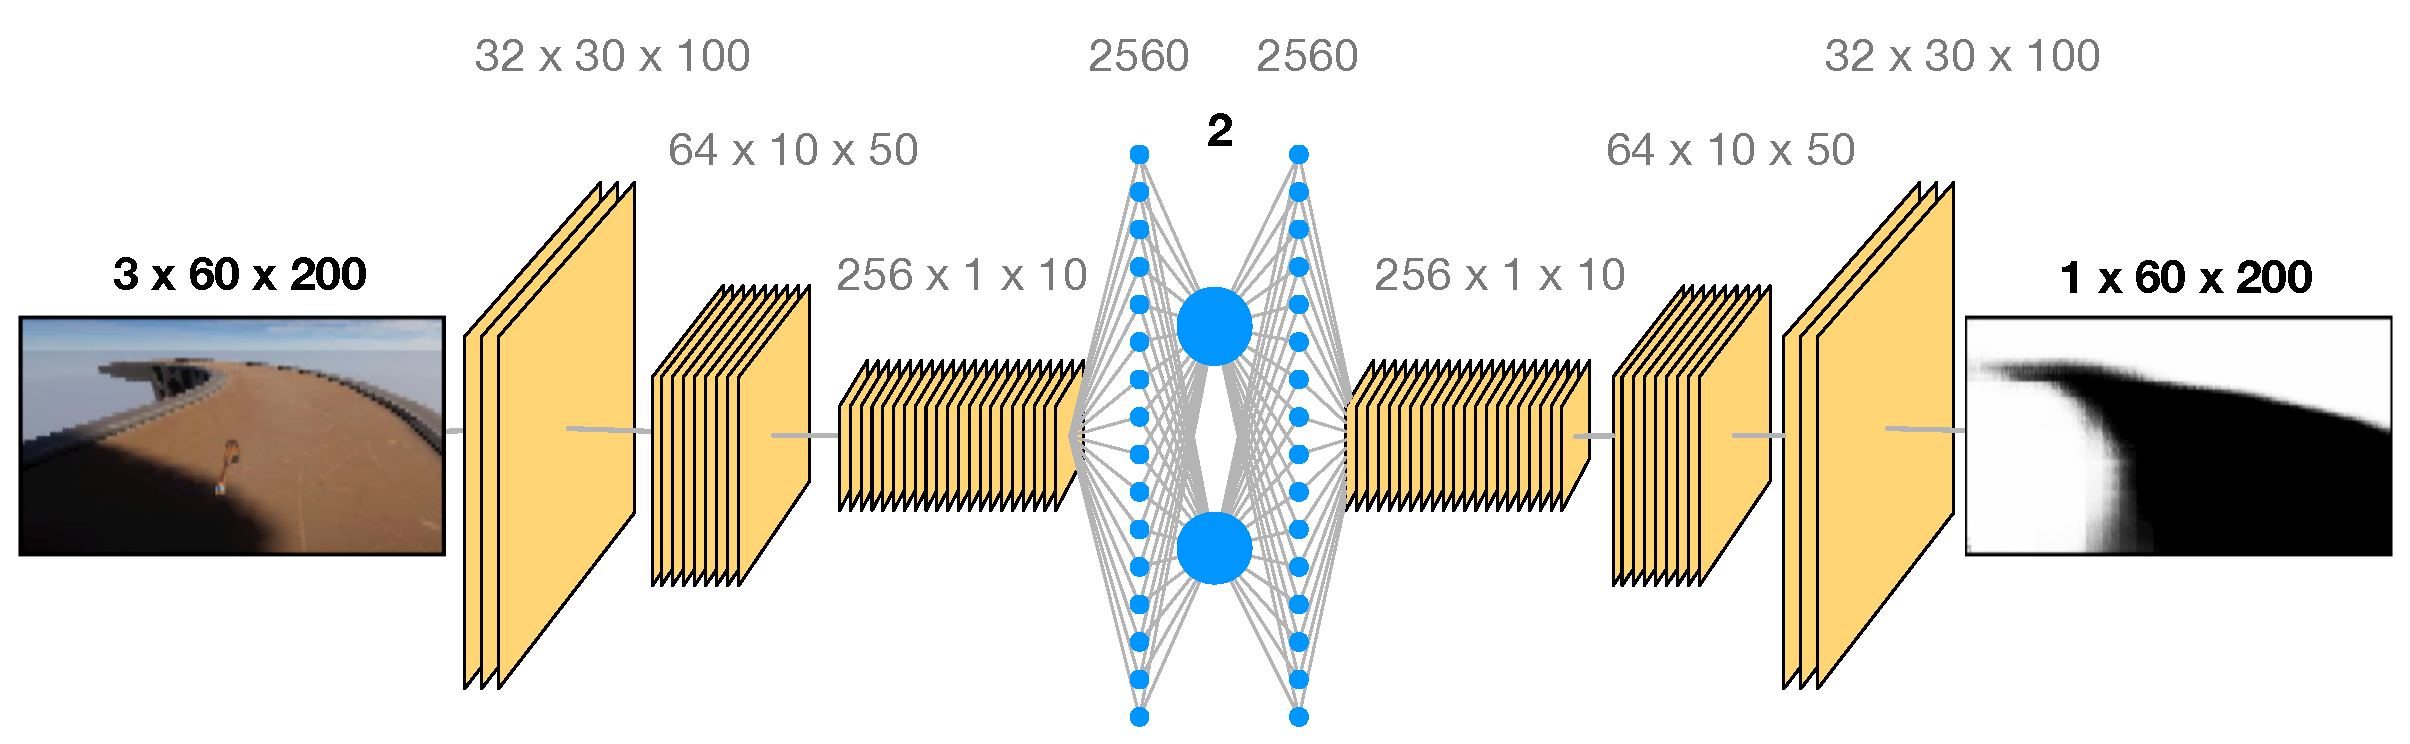
\includegraphics[width=1.0\linewidth]{images/VAE_Segmentation.eps}
  \caption{Encoder Decoder structure with 2 features in the bottleneck layer for image segmentation.}
\label{fig:segmentation_encoder-decoder}
\end{figure}

\subsection{VAE Segmentation - Results}
Training with the Unity game in normal mode (not headless) runs a bit slower. Two million steps took 48 hours. However, the learning curve of the agent is significantly shallower with the two new image features. Presumably, the features are too unstable or not sufficiently expressive. With the result after 2M steps, the agent reaches the end of level 1. A video of the training agent can be found here  https://youtu.be/eW7DPDBPcZs. The agent can be seen as a proof of concept, but in order to play the game with it, further development is needed.

\begin{figure}[!t]
\centering
\includegraphics[width = 1.0\linewidth]{images/Level_1_ep_rew_mean_VAE_segmentation.eps}
\caption{SAC training curves graphical agent.}
\label{fig:SAC01learningcurvVAEsegmentation}
\end{figure}

\subsection{Classic image preprocessing as feature extractor} \label{Classic_image_preprocessing_as_feature_extractor}
% TODO: Michelle
In order to simplify feature extraction from the images preprocessing is required.

In the first attempt the watershed method suggested in \cite{Watershed} and \cite{Watershed2} was to used. It segments the image to differentiate between objects. The result of the method is shown in the \figurename  \ref{fig:watershed}. Watersheding is able to distinguish the trees from the path in the RoboSkate game, what is necessary for the further calculations. The disadvantage of this method is the calculation time for a is single image. It takes on average 5 seconds without adding any learning, yet. Therefore, this method proves to be impractical in runtime of the game. 

\begin{figure}[!t]
\centering
\includegraphics[width = 1.0\linewidth]{images/Michelle_object_detection.png}
\caption{Results of using the watershed method on RoboSkate.}
\label{fig:watershed}
\end{figure}

Another approach was suggested in \cite{ImageProcessing} and \cite{Canny}. First, a noisy image is created, which is then fed through a canny filter. In \figurename  \ref{fig:preprocessingcomparision} contains the results. Three different results were created. One with the noisy image, where the canny filter was not used. Then the canny filter was applied with the scale factor $\sigma = 1$ and $\sigma = 3$. We can see when the scale factor $\sigma = 1$ the result is not as smooth as when $\sigma = 3$. As with the scale factor $\sigma = 3$ a better outcome is achieved, it will be utilized from now on. The appearing question is, if the noisy image or the canny filter is giving the better results. 

\begin{figure}[!t]
\centering
\includegraphics[width = 1.0\linewidth]{images/Preprocessing_Comparision.png}
\caption{Comparison of different methods for image preprocessing on RoboSkate.}
\label{fig:preprocessingcomparision}
\end{figure}

In order to test this, the DummyBall environment was used, as it is a simpler version of the game and therefore faster in learning. The results of applying the two methods is shown in \figurename  \ref{fig:dummyballcanny} and \ref{fig:dummyballnoisy}.

\begin{figure}[!t]
\centering
\includegraphics[width = 1.0\linewidth]{images/DummyBall_Canny.png}
\caption{Results on using the canny filter method on DummyBall.}
\label{fig:dummyballcanny}
\end{figure}

\begin{figure}[!t]
\centering
\includegraphics[width = 1.0\linewidth]{images/DummyBall_Noisy.png}
\caption{Results of using the noisy method on DummyBall.}
\label{fig:dummyballnoisy}
\end{figure}

As a learning algorithm the PPO algorithm is utilized. In \figurename  \ref{fig:dummyballresultslocation} the location of the DummyBall is plotted over 20000 steps. In the graphic the violet graph is representing the canny filter method and the yellow one aroused with using the noisy images. As seen in this figure, the difference of these two image preprocessing methods is significant. While using the canny filter method, the agent starts slowly learning at around 1600 time steps, whereas the agent with the noisy images starts learning significant at 8000 time steps. 

\begin{figure}[!t]
\centering
\includegraphics[width = 1.0\linewidth]{images/DummyBall_Results1.jpg}
\caption{Comparison of the results from the canny filter and the noisy method of the location from DummyBall.}
\label{fig:dummyballresultslocation}
\end{figure}

As the noisy method works significantly better, it will be considered in the further process. The method applied on RoboSkate can be seen in \figurename  \ref{fig:NoisyRoboSkate}. With the color differences in the noisy images, the desired turning angle could be calculated. The robot then used the calculated turning angle to get through the parkour. 

%\begin{figure}[!t]
%\centering
%\includegraphics[width = 1.0\linewidth]{images/DummyBall_Results2.jpg}
%\caption{Comparison of the results from the canny filter and the noisy method of the reward from DummyBall.}
%\label{fig:dummyballresultsreward}
%\end{figure}



\begin{figure}[!t]
\centering
\includegraphics[width = 1.0\linewidth]{images/Preprocessing12.png}
\caption{Result of the noisy method on RoboSkate.}
\label{fig:NoisyRoboSkate}
\end{figure}


%\begin{figure}[!t]
%\centering
%\includegraphics[width = 1.0\linewidth]{images/Methodenschritte2.png}
%\caption{Steps of Preprocessing}
%\label{fig:StepsPreprocessing}
%\end{figure}

Some problems occurred with this method. One is shown in \figurename  \ref{fig:problemspreprocessing}. At one certain point in level 1, the color code of the preprocessing changed. The road suddenly became the obstacle. This problem could be solved with a dynamic change of which color gets seen as an obstacle.

\begin{figure}[!t]
\centering
\includegraphics[width = 1.0\linewidth]{images/Preprocessing14.png}
\caption{Problems of the preprocessing.}
\label{fig:problemspreprocessing}
\end{figure}

All in all does this preprocessing method work for level 1. The robot takes in average 4:30 min to complete level 1 and around 1800 images are needed. 

%\begin{figure}[ht]
%\centering
%\includegraphics[width = 1.0\linewidth]{images/Preprocessing15.png}
%\caption{Problems of the preprocessing 2.}
%\label{fig:problemspreprocessing2}
%\end{figure}

\section{Combined Policy}
The disadvantage of all the attempts presented so far is that no end to end reinforcement learning takes place but individual parts are always trained separately. With a trainable feature extractor that first treats image data and numerical data separately and then combines them in a common policy, the problem could be solved.

Such a multi input policy with combined feature extractor has been implemented and tested as shown in \figurename  \ref{fig:Combined_Policy}. Since this training requires a lot of server resourses, no agent has been trained yet. The copying of already trained layers from the previous networks could also be tried out in the future and possibly lead to an agent that could learn further levels completely autonomously.

\section{Server training}
The networks used for behavioral cloning, described in section \ref{Segmentation_training} and \ref{Behavioral_cloning}, could be trained directly on local machines. The reinforcement learning algorithms were much more time consuming and required the use of servers.
\figurename  \ref{fig:Server_struktur} shows the interconnection of the two servers as used for our first training sessions.

\subsection{Vectorized Environment}
To train in parallel on multiple environments, a vectorized environment was created, which can be started with any number of instances of the RoboSkate game.

It is also possible to run RoboSkate instances that are not executed on the same machine but are instead being launched remotely.
The Gym environments serve as wrappers to provide RoboSkate with the widely used OpenAI Gym interface. Communication between the Gym Environments and the RoboSkate instances is done using gRPC. For RoboSkate instances running remotely, there must also be an ssh connection to the machine through which gRPC is used to communicate. In this case, only RoboSkate runs remotely, the Gym Wrapper remains on the local machine. \figurename  \ref{fig:Vectorized_Environment} shows the schematic structure of the Vectorized Environment. It should be noted that one RoboSkate instance can be avoided for evaluation by reusing an instance from training. Since there is no training during the evaluation and the environment is reset at each episode, there is no overlap in usage.
Since only one server is equipped with GPUs, and the bottleneck at the training are the RoboSkate Unity instances, the distribution over the network could not provide any performance advantage.

\begin{figure}[!t]
  \centering
  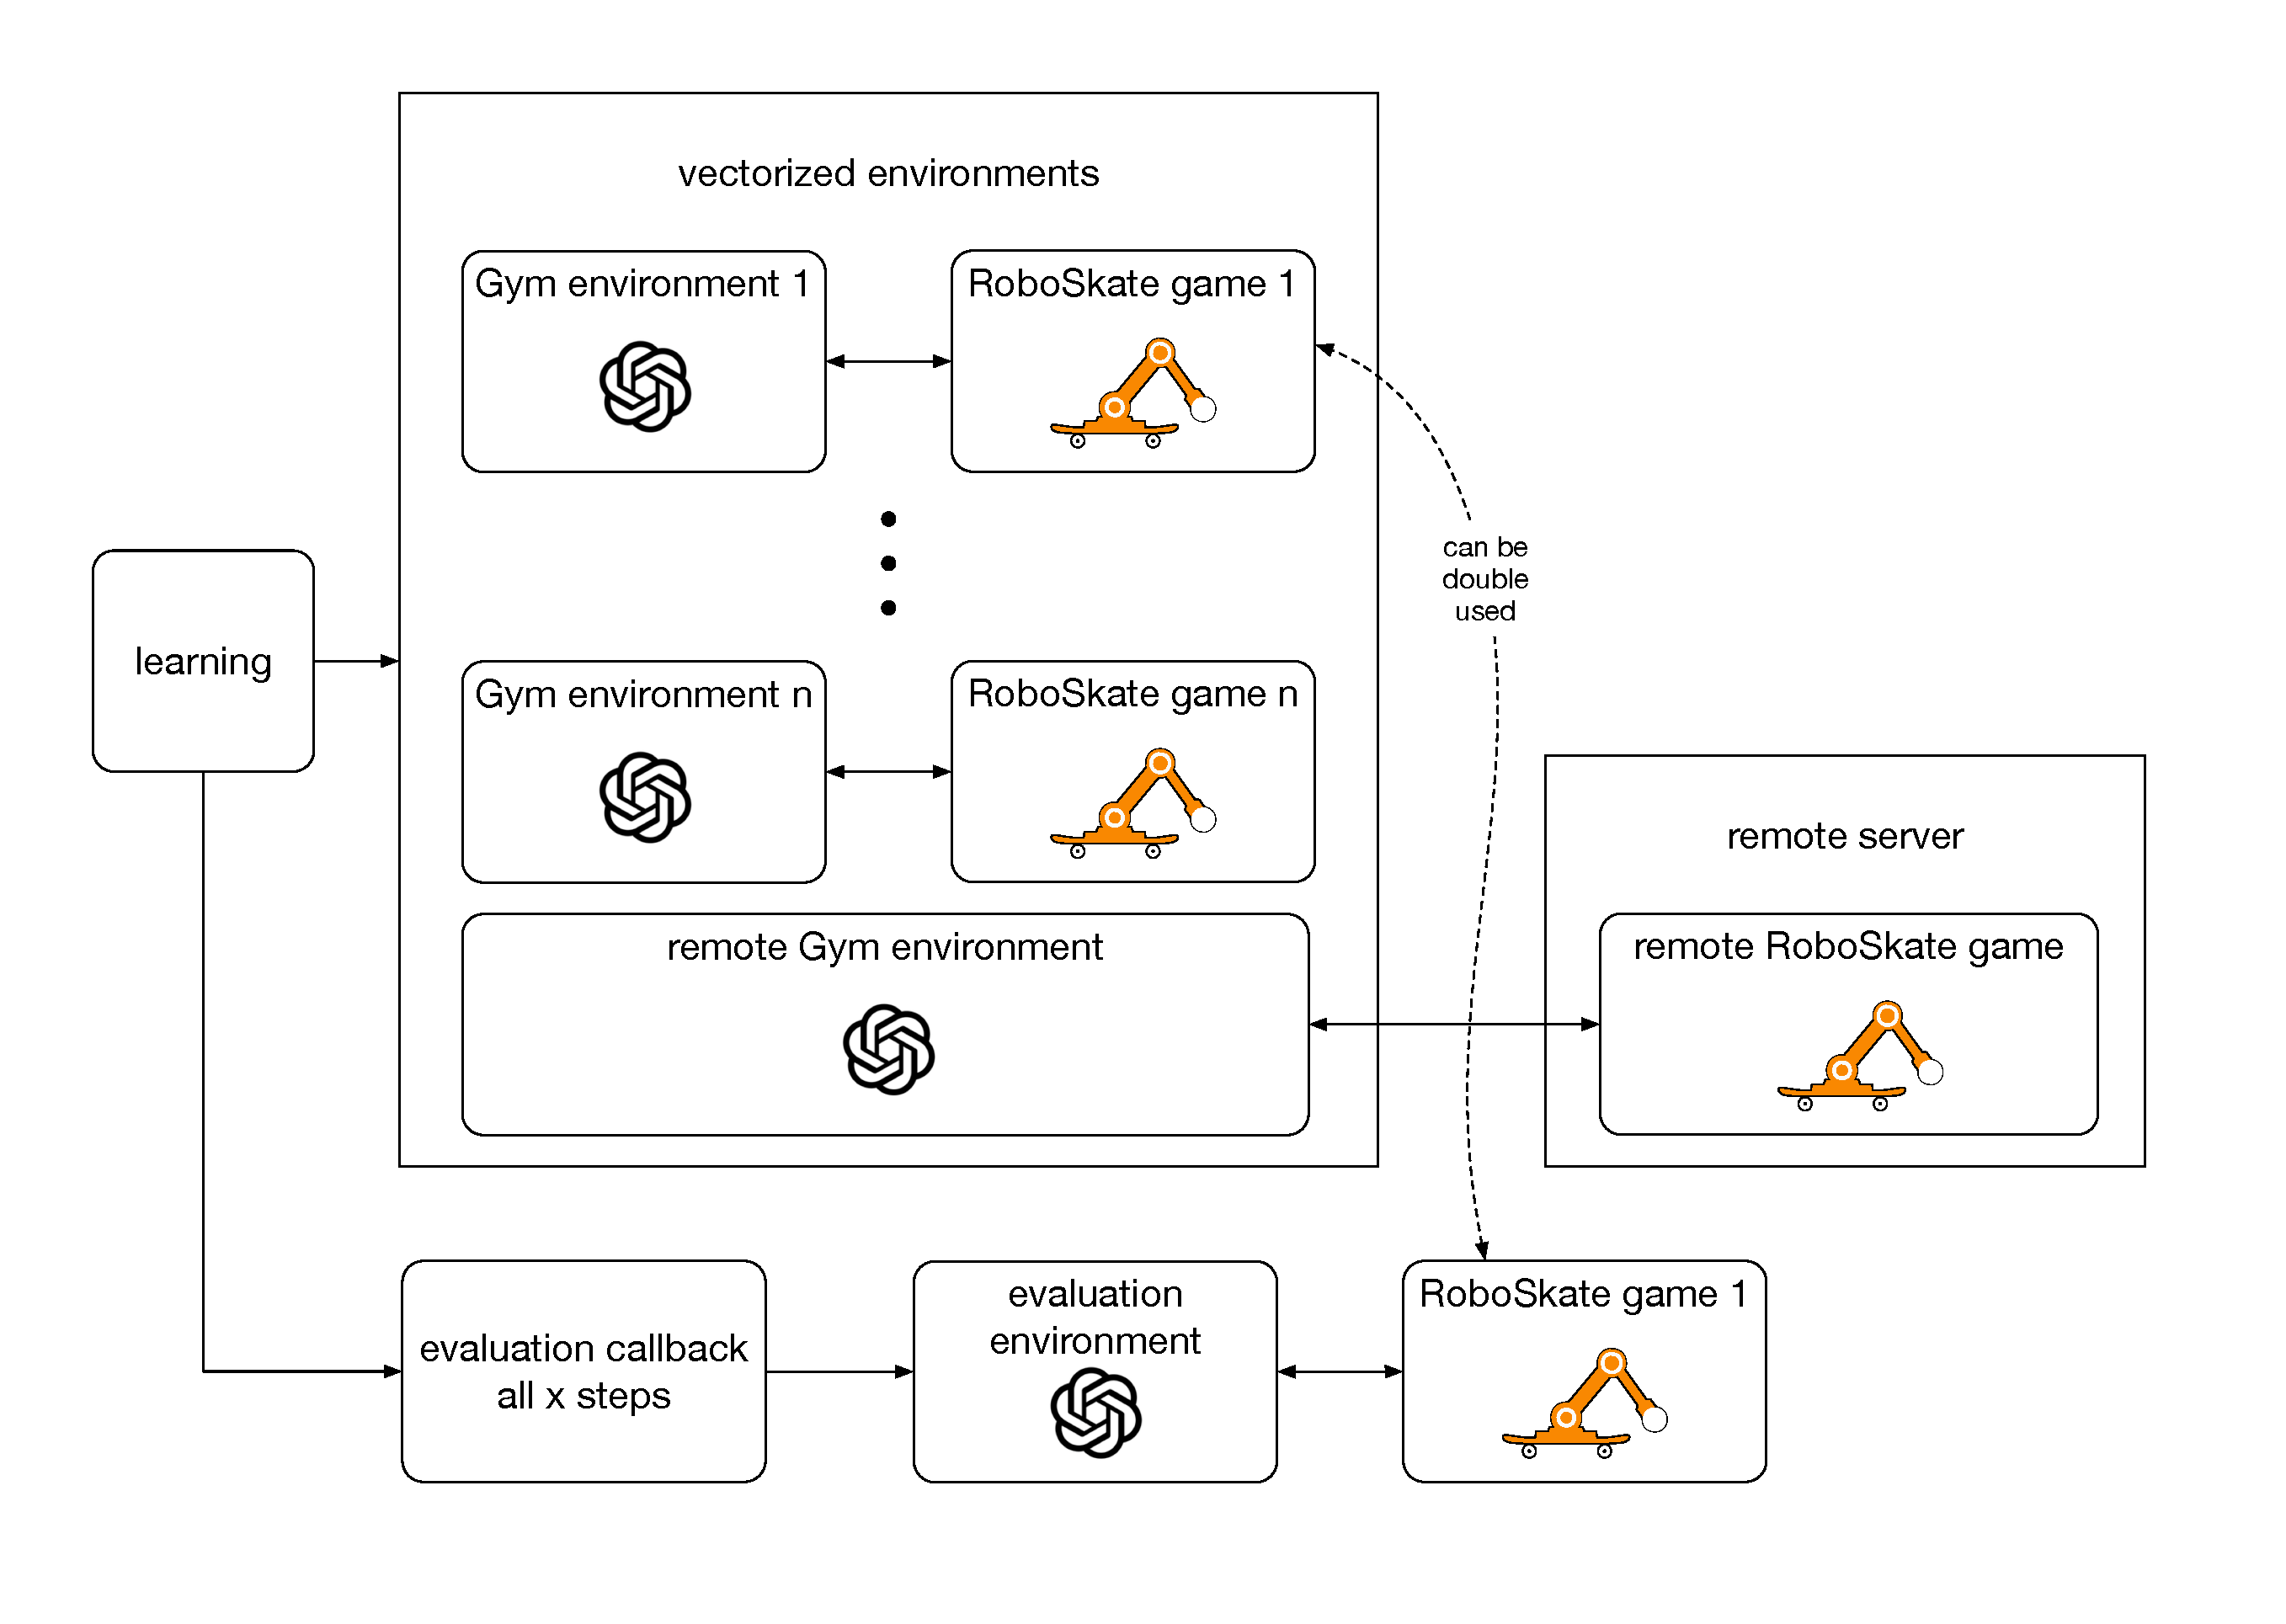
\includegraphics[width=1.0\linewidth]{images/Vectorized_Environment.eps}
  \caption{Vectorized Environment.}
\label{fig:Vectorized_Environment}
\end{figure}

%\section{Comparison with human players}
% TODO: Batu
%Already on the first meters you can see how the agent outperforms an untrained human player. A comparison with trained players was made by using let's plays from YouTube. However, since there is a shortcut directly between level 1 and level 3, and the agent has been trained level wise, there is no way for it to have found it. Since the first level takes a relatively long time, many players have also spend a substantial part of their videos there. Therefore, only the RoboSkate Developer playthrough by Matas Sakalauskas \cite{Playthrough}, the game developer, can really be used as a benchmark.

%\figurename  \ref{fig:Benchmarking} reveals time comparison of the numerical agent and different human players. Y axis represents the time in seconds and the colors represent the breakdown of each level. An inexperienced new player needs around 3 hours training to reach the end of level three in 5 minutes. The learning process of the new player can be seen \href{https://youtu.be/08u6hHvOCj0}{here}. The developer of the game can finish the game in 3 minutes with an experience of more than a year. A speed runner from YouTube with unknown hours of training can complete all three levels in 2 minutes. The \href{https://www.youtube.com/watch?v=xL9v7Ss90LU}{game play} can be seen here. The trained agent, however, can finish the game in 50 seconds.

%\begin{figure}[!t]
%  \centering
%  \includegraphics[width=1.0\linewidth]{images/human_benchmarking.png}
%  \caption{Comparison of the numerical agent with human players.}
%\label{fig:Benchmarking}
%\end{figure}

%It should be also mentioned that the agent can neither use the magnet, which is used for climbing, nor the possibility to reset the robot at the right moment. Both are techniques that are used by professional players in higher levels. One advantage that the agent may have against the human players is the joint force, because it's limits are unknowned in the game. The force limit in our setting is only an estimate. With higher values, the agent can complete, especially the first level, even faster.

%As has been clearly shown, the agent finishes the levels much faster than a human player. One disadvantage, however, is the training time. A human immediately understands how to move the robot forward. Depending on the initial pose, the agent needs several hours until it can make a first directed movement. 

%\begin{center}
%\begin{table}
%\centering
% \begin{tabular}{l c c c} 
% \hline
%& Level 1 & Level 2 & Level 3 \\ 
% \hline\hline
%Matas Sakalauskas &  115 & 42 & 25 \\ 
% \hline
%Numerical agent & 32 & 12 & 6 \\
% \hline
%\end{tabular}
%\caption{Level times comparison in seconds.}
%\label{table:Timecomparison}
%\end{table}
%\end{center}

%For future experiments it could be interesting to extend the action space. It would also be interesting to change the reward function so that the agent can find the shortcut between level 1 and 3. However, this requires a lot of training and is probably unlikely with the resources.

\section{DummyBall Game}
% Gin
We were also provided with a simpler version of the RoboSkate environment called DummyBall game (\figurename  \ref{fig:dummyballcanny}), which served as a platform to easily test our implementations. It is a game where the player controls a ball with left and right arrow keys, while it rolls forward. The goal is to reach the end of the track by avoiding falling off. 

In the early stages of our development, we learned a few key concepts when using reinforcement learning on this game that we brought over to the RoboSkate game. First, consistent termination of an episode leads to faster learning (influenced \ref{Termination_conditions}). In the DummyBall game the platform is not aligned with the global coordinate system, which is used as a reference point for the agent observations, and is a about 2 degrees off. This resulted in the ball falling farther before terminating the episode in the farther section of the track compared to the early part of the track. Second, smaller preprocessed simpler images are easier for the algorithm to learn from (influenced \ref{Classic_image_preprocessing_as_feature_extractor}, \ref{VAE_Segmentation}). The grayscale version of the 150x150 size image with Canny filter applied (\figurename  \ref{fig:DB_canny}) proved to be the fastest to converge during the learning process of PPO and A2C. We assume it is, because the track was fully visible and distinguishable from the background elements (\figurename  \ref{fig:DB_conv}). Third, the average performance of the agents is a more accurate estimate of performance. The learning results depend on the initialization of the agent, it is especially true when using A2C (\figurename  \ref{fig:DB_A2C}). 

% Subfigures according to "A. Figures 1)"

\begin{figure}[!t]
\centering
\subfloat[Original observation image.]{\includegraphics[width=0.2\textwidth]{images/DB_canny.png}
\label{fig:DB_canny}}
\hfil
\subfloat[After convolution layers.]{\includegraphics[width=0.2\textwidth]{images/DB_conv.png}
\label{fig:DB_conv}}
\caption{Image provided as an observation for the DummyBall agent.}
\end{figure}

\begin{figure}[!t]
  \centering
  \includegraphics[width=1.0\linewidth]{images/A2C_randomness.png}
  \caption{Smoothed performance graph of 3 instances of A2C agent in the DummyBall game. The maximum reachable distance before termination is 60.}
\label{fig:DB_A2C}
\end{figure}

\section{NRP}
% Gin
After the work mention above the goal was to transfer everything in to a docker image for simple and fast distribution and run the algorithms with the help of NeuroRobotic Platform (NRP). We were provided with a docker image hbpneurorobotics/nrp-core:unity, which contained already the NRP. In order to use our implementation in the docker container necessary libraries needed to be installed like Stable baseline 3 (SB3). 

Running NRP together with SB3 proved to be difficult. Firstly, unable to pass data from NRP Script class directly to SB3, because it's class instance is initialized inside NRP during runtime, so the class instance is not reachable from SB3. Secondly, "restart" and "shutdown" methods were not implemented, that are required for resetting the gym environment after termination conditions are met or closing the application. So basically only an already trained agent could be run with this setup. Furthermore, importing libraries globally did not work and only local import proved to work. 

A workaround for the first problem was implemented that uses gRPC communication protocol to establish a communication channel through a system's port to enable data exchange between NRP and SB3. Because the information swap was taking place in the NRP class loop method "runLoop" and SB3 step loop, a third class was considered, which would take a role as a server and handle the data distribution between subscribers e.g. NRP and SB3 (\figurename  \ref{fig:NRP_docker}).

With this setup it was possible to run a trained PPO agent with the NRP DummyBall game in a docker container, but some drawbacks were also discovered. The first thing that could be notices was, that the agent was behaving differently then learned and was not able to reach the end of the track. Furthermore, some synchronization problems arose. NRP simulation was running faster then the agent was trained for. We assume that is why the behavior of the agent changed. After trying to add timers to synchronize the loops no successful combination of timeouts was found. Because NRP is still in development, the next version could contain solutions to the problems described above. So therefore no further explorations of the problems were done.

\begin{figure}[!t]
  \centering
  \includegraphics[width=1.0\linewidth]{images/NRP_docker.png}
  \caption{Communication architecture of NRP and SB3 in the docker container.}
\label{fig:NRP_docker}
\end{figure}


\section{Final result}
% TODO: Batu
The numerical agent can significantly outperform a human player. The agent requires 50 seconds to complete all three levels. To achieve that performance the agent is trained for more than 20 hours and 1 million steps based on a previously trained model for 10 hours. \href{https://youtu.be/eR-Nq7dy4qw}{Final performance of the numerical agent} can be seen here. \figurename  \ref{fig:Tensorboard} illustrates the learning graph. Y axis shows the mean reward and X axis shows the number of steps.

\begin{figure}[!t]
  \centering
  \includegraphics[width=1.0\linewidth]{images/tensorboard_2_smooth.png}
  \caption{Learning Graphic of the Numerical Agent.}
\label{fig:Tensorboard}
\end{figure}

\figurename  \ref{fig:Benchmarking} reveals time comparison of the numerical agent and different human players. Y axis represents the time in seconds and the colors represent the breakdown of each level. An inexperienced new player needs around 3 hours training to reach the end of level three in 5 minutes. The learning process of the new player can be seen \href{https://youtu.be/08u6hHvOCj0}{here}. Matas Sakalauskas \cite{Playthrough}, the game developer, can finish the game in 3 minutes with an experience of more than a year. A speed runner from YouTube with unknown hours of training can complete all three levels in 2 minutes. The \href{https://www.youtube.com/watch?v=xL9v7Ss90LU}{game play} can be seen here. The trained agent, however, can finish the game in 50 seconds.

\begin{figure}[!t]
  \centering
  \includegraphics[width=1.0\linewidth]{images/human_benchmarking.png}
  \caption{Comparison of the numerical agent with human players.}
\label{fig:Benchmarking}
\end{figure}

It should be also mentioned that the agent can neither use the magnet, which is used for climbing, nor the possibility to reset the robot at the right moment. Both are techniques that are used by professional players in higher levels. One advantage that the agent may have against the human players is the joint force, because it's limits are unknown in the game. The force limit in our setting is only an estimate. With higher values, the agent can complete, especially the first level, even faster.

For future experiments it could be interesting to extend the action space. It would also be interesting to change the reward function so that the agent can find the shortcut between level 1 and 3, which the high-level human players use to save significant amount of time. However, the agent has been trained level wise, there is no way for it to have found it. Moreover, this requires a lot of training and is probably unlikely with the resources.

\section{Future Work}
In further work, especially the learning from image data is interesting. How can more robust features be extracted that provide a clearer sense of direction? Can a VAE be trained that learns from non-labeled images and can still generalize sufficiently in the environment? Or can even a policy be learned which actually learns from the image input?

The reward function could also be redesigned. Does it need so many checkpoints? Could a penalty per step be introduced so that the agent learns to get to the goal as quickly as possible? Currently, the agent learns to move faster by covering as much distance as possible per time step (higher reward). At the same time, it also optimizes the trajectory to be as accurate as possible.


% ========== Start of Bibliography ==========
% according to  "C. Bibliographies" from the rule book

\bibliographystyle{IEEEtran}
\bibliography{IEEEabrv,roboskate_bib}

% ========== Start of appendix ==========

\newpage
\onecolumn
\appendix

% tables according to "C. Tables"

\begin{table*}[ht!]
    \renewcommand{\arraystretch}{1.3}
    \caption{Video links}
    \centering
    \begin{tabular}{l l} 
        \hline
        Numerical agent 1 & https://youtu.be/fPrDSwJhh1M \\ 
        \hline
        Segmentation results during teleoperation &  https://youtu.be/j55lKt12hTM \\ 
        \hline
        Hardcoded agent simulation & https://youtu.be/TBJDABXq6XM \\
        \hline
        Behavioral Cloning & https://youtu.be/xmD-cCVVcfk \\
        \hline
        RoboSkate teleoperation and image reconstruction & https://youtu.be/j55lKt12hTM \\
        \hline
        Graphical agent with two features from segmentation & https://youtu.be/eW7DPDBPcZs \\
        \hline
        Model trained on level 2 finishes level 3 (Numerical) & https://youtu.be/y-slDJ-4uvA\\
        \hline
        Agent without limitations learn to pull (Numerical) & https://youtu.be/s-T2NOSyQ6g\\
    
    \end{tabular}
\end{table*}

% tables according to "C. Tables"

\begin{table*}[ht!]
    \renewcommand{\arraystretch}{1.3}
    \caption{All observations which can be retrieved from RoboSkate.}
    \label{tab:all_observation}
    \centering
    \begin{tabular}{c|c|c|c|p{6cm}}
        \textbf{variable}  & \textbf{description}  & \textbf{range}  & \textbf{unit}  & \textbf{comment} \\
        \hline
        \hline
        boardCraneJointAngles[0] & Joint1 pos. & [-180, 180] & deg  &   \\
        boardCraneJointAngles[1] & Joint2 pos. &  [-90, 90]  &  deg &    \\
        boardCraneJointAngles[2] & Joint3 pos. &  [-125, 125]  &  deg &    \\
        boardCraneJointAngles[3] & Joint1 velocity &  [-170, 170]  &  deg/sec  & inputAction * 3,67 = outputVelocity \\
        boardCraneJointAngles[4] & Joint2 velocity &  [-170, 170]  &  deg/sec  & inputAction * 3,67 = outputVelocity \\ 
        boardCraneJointAngles[5] & Joint3 velocity &  [-170, 170]  &  deg/sec  & inputAction * 3,67 = outputVelocity \\
        \hline
        boardPosition [0] &  x  &  [-220, 220]  &  m  &  forward / backward\\
        boardPosition [1] &  z  &  [-20, 20]  &  m  &  up / down \\
        boardPosition [2] &  y  &  [-220, 220]  &  m  &  left / right \\
        boardPosition [3] &  Velocity x  &  [-10, +10]  &  m/sec  &  \\
        boardPosition [4] &  Velocity z  &  [-10, +10]  &  m/sec  & \\
        boardPosition [5] &  Velocity y  &  [-10, +10]   &  m/sec  & \\
        boardPosition [6] &  Acceleration x  &  [-10, +10]  &  rad/sec  & Very unstable. Not recommended to use. \\
        boardPosition [7] &  Acceleration z  &  [-10, +10]  &  rad/sec  & Very unstable. Not recommended to use. \\
        boardPosition [8] &  Acceleration y  &  [-10, +10]  &  rad/sec  & Very unstable. Not recommended to use.\\
        \hline
        boardRotation [0] - [2] &  Euler  &  [0, 360]  &  deg  &  no meaningful output.  \\
        boardRotation [3] - [6] &  Quaternion &  [-1, 1]  &  & no meaningful output.  \\
        boardRotation [7] &  forward x  &  [-1, 1]  &    &   If the board is pointing straight forward, this entry is 1.  \\
        boardRotation [8] &  forward z &  [-1, 1]  &    &  If the entry is 1, the board is vertically upright (so hopefully never). \\
        boardRotation [9] &  forward y &  [-1, 1]  &    &  If the board points to the left, this entry is 1.  \\
        boardRotation [10] &  upward x  &  [-1, 1]  &    &  If the board were pitched or rolled (depending on the Yaw) 90°, this value would be 1.   \\
        boardRotation [11] &  upward z  &  [-1, 1]  &    &  When the Bold is flat on the ground this entry is 1 (yaw dose not change this value)  \\
        boardRotation [12] &  upward y  &  [-1, 1]  &    &  If the board were pitched or rolled (depending on the Yaw) 90°, this value would be 1. If it is rolled in initial position this is 1.   \\
    \end{tabular}
\end{table*}

\begin{figure*}[ht!]
  \centering
  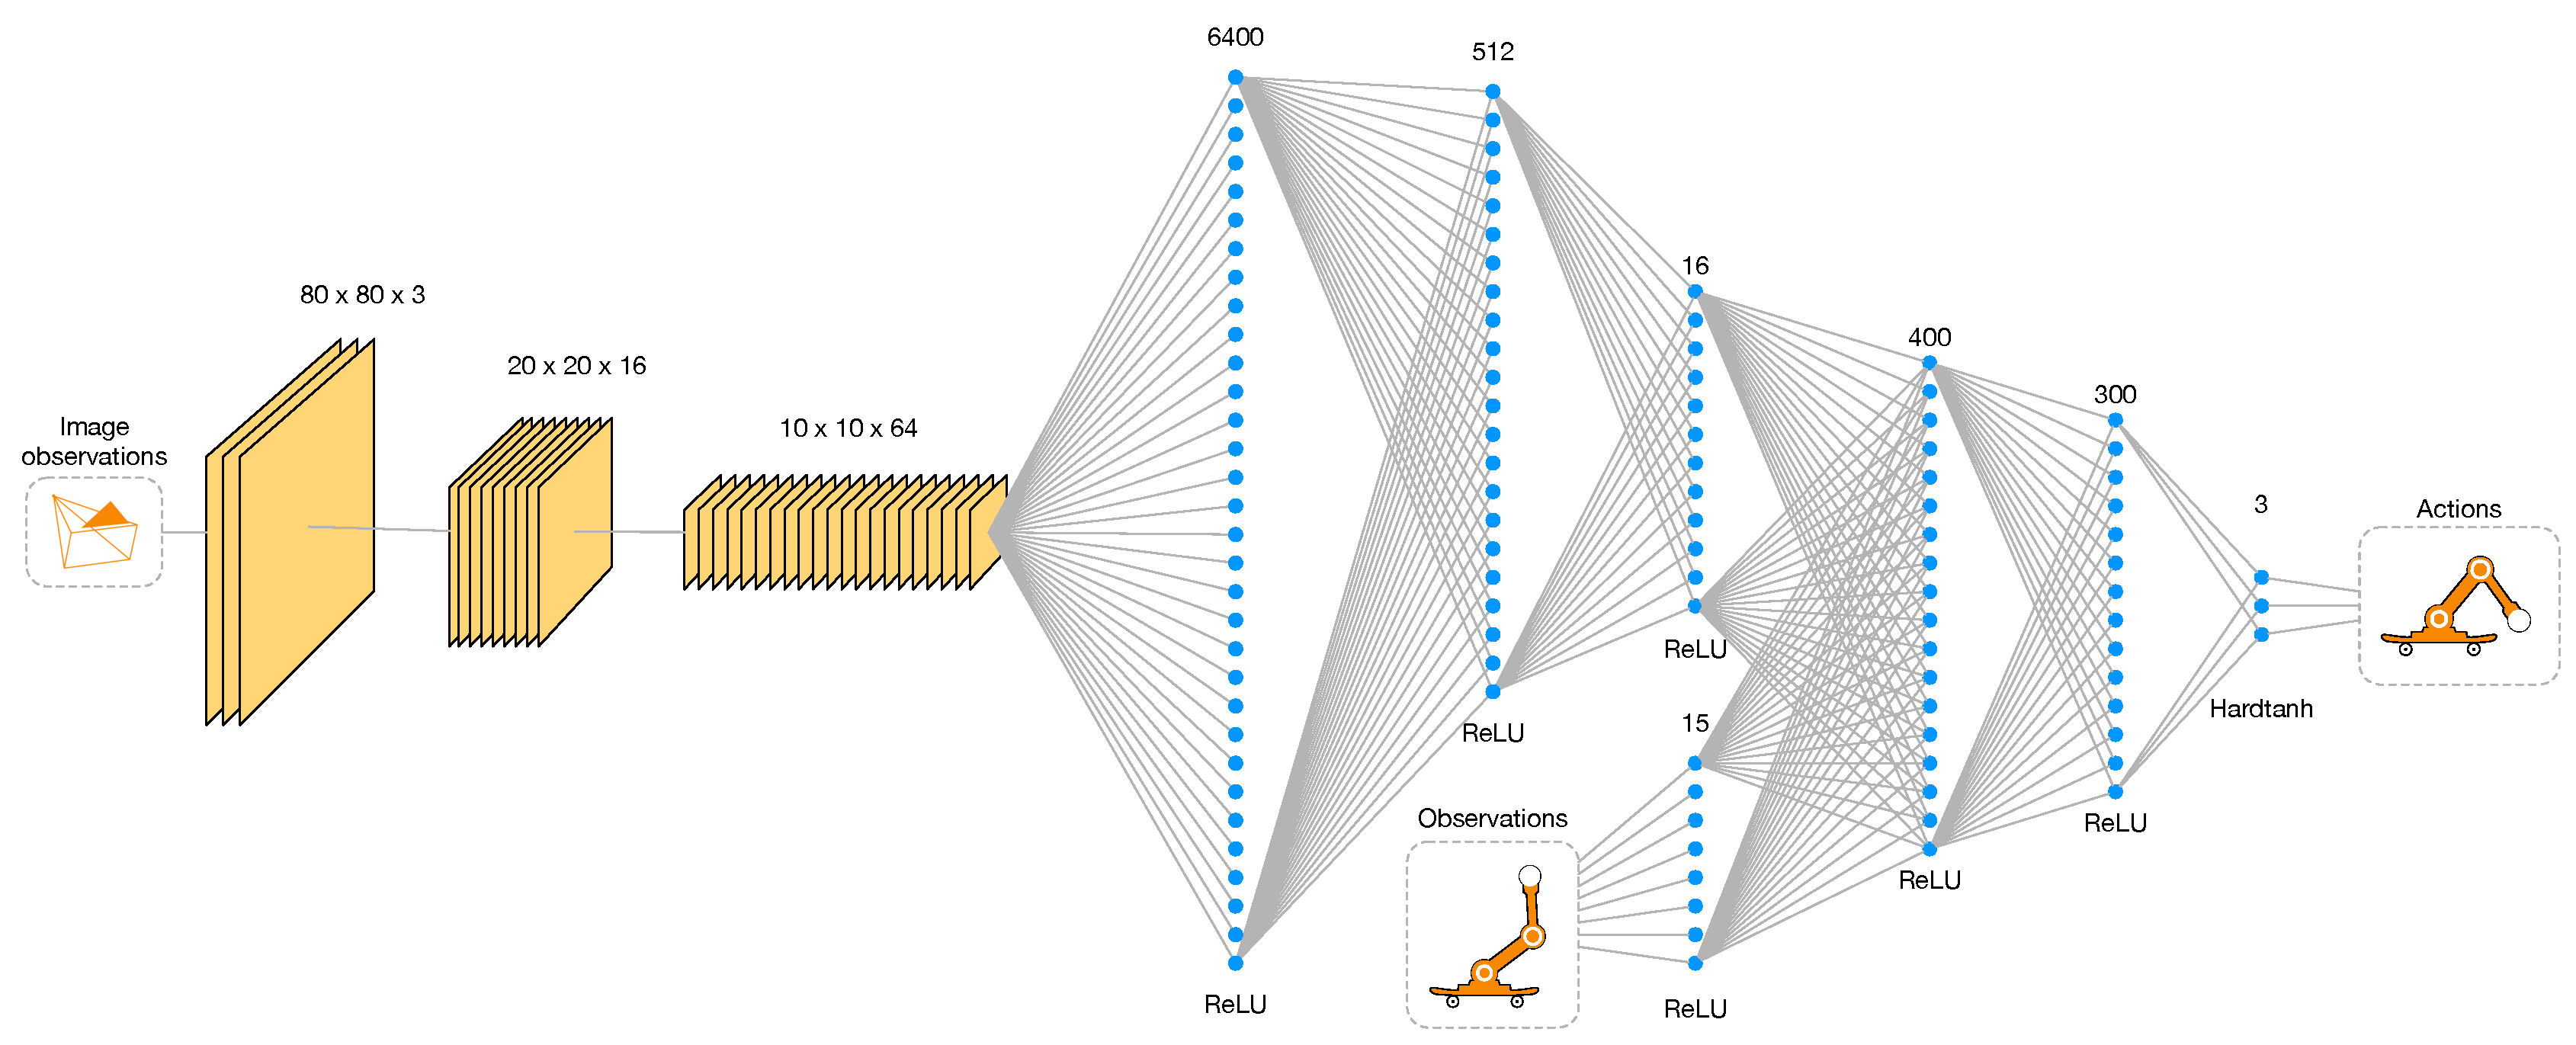
\includegraphics[width=1.0\linewidth]{images/Learning_from_images_Policy.eps}
  \caption{Combined feature extractor to also learn the image processing directly with the RL algorithm.}
\label{fig:Combined_Policy}
\end{figure*}

\begin{figure*}[ht!]
  \centering
  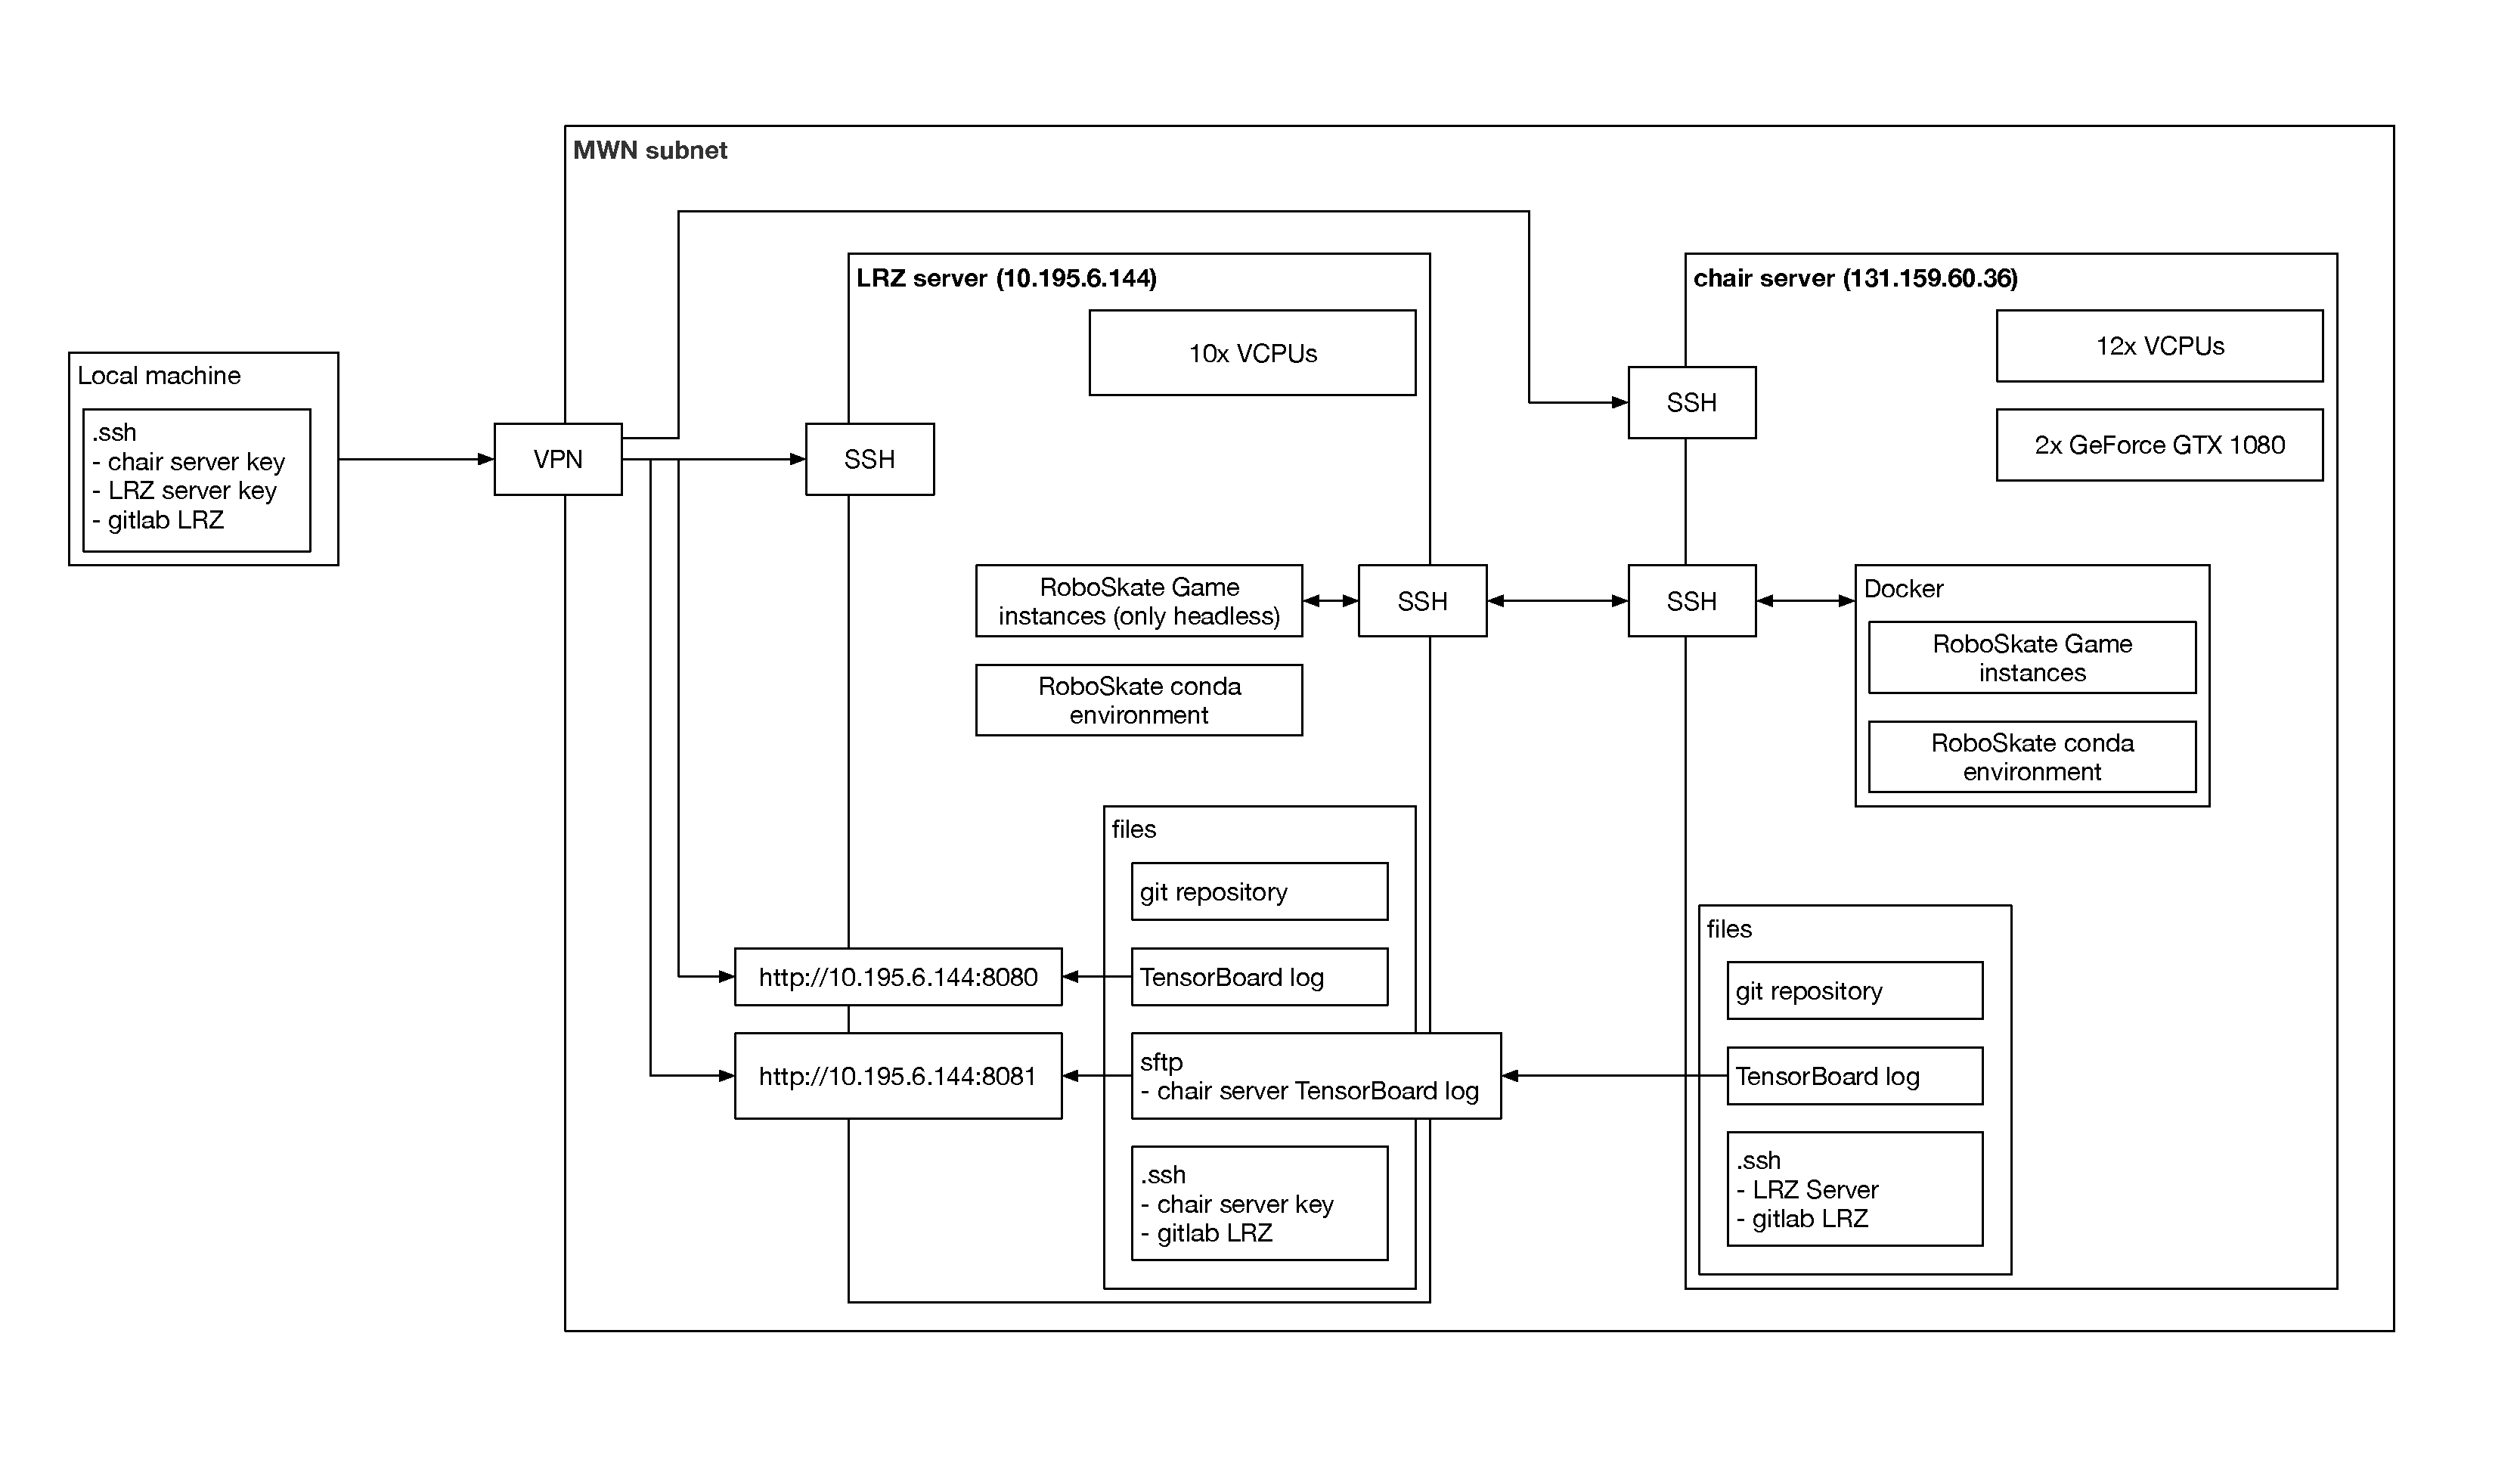
\includegraphics[width=.9\linewidth]{images/Server_struktur.eps}
  \caption{Server architecture used for training.}
\label{fig:Server_struktur}
\end{figure*}



\end{document}
%\caption{Comparison of the results from the canny filter and the noisy method of the reward from DummyBall}

